\chapter{球対称質量モデルと数値積分}
\label{chap:numint}

銀河や星団のような自己重力系を記述するとき、最初に必要になる量の一つが、密度分布から求める内包質量（enclosed mass）である。
球対称な密度分布 $\rho(r)$ が与えられれば、半径 $r$ より内側の質量は積分で求められる。
しかし、密度分布が複雑になると積分を解析的に実行できるとは限らない。
そこで本章では、Ryden §6.4 の球対称質量モデルを題材として、\textbf{数値積分（numerical integration）}の基本を学ぶ\cite{ryden2025}。

中心となる例は Plummer 球である。
Plummer 密度分布では内包質量を解析的にも求められるため、数値積分の答えがどの程度正しいかを直接確認できる。
このように、\textbf{解析解が分かる問題を数値計算法の検証に使う}ことは、以後の章でも繰り返し用いる基本的な考え方である。

\begin{learningbox}[本章で学ぶこと]
\begin{itemize}
\item 球対称な密度分布から内包質量を求める問題について、数値積分の被積分関数と積分区間を設定できる。
\item 左長方形則、中点則、台形則、Simpson 則の近似の考え方を説明し、Python で実装できる。
\item 累積積分を用いて、積分上限が異なる複数の積分値を効率よく計算できる。
\item 解析解との比較と格子収束試験から、各積分公式の誤差と収束次数 $p$ を評価できる。
\item 離散化誤差と丸め誤差を区別し、格子を細かくしても精度が向上しなくなる理由を説明できる。
\end{itemize}
\end{learningbox}

本章に対応する数値実験は、Notebook 1「球対称質量モデル」で行う。
本文中の Listing には、導いた公式に対応する短い Python コードを示す。計算全体を実行して結果を図にするコードは Notebook にある。

\section{球対称密度分布と内包質量}
\label{sec:ch1-spherical-mass}

\subsection{球殻の質量要素}

球対称な密度分布を $\rho(r)$ とする。
半径 $r$、厚さ $dr$ の薄い球殻の体積は
\begin{equation}
 dV = 4\pi r^2\,dr
\label{eq:ch1-shell-volume}
\end{equation}
であるから、その球殻に含まれる質量は
\begin{equation}
 dM = \rho(r)\,dV
 = 4\pi r^2\rho(r)\,dr
\label{eq:ch1-shell-mass}
\end{equation}
である。
したがって、半径 $r$ より内側の\textbf{内包質量（enclosed mass）}は
\begin{equation}
 \boxed{
 M(<r)=\int_0^r 4\pi\rho(r')\,r'^2\,dr'
 }
\label{eq:ch1-enclosed-mass}
\end{equation}
となる。

ここで数値積分するのは $\rho(r)$ そのものではなく、
\begin{equation}
 f_M(r)\equiv \frac{dM}{dr}=4\pi r^2\rho(r)
\label{eq:ch1-mass-integrand}
\end{equation}
である。
半径 $r$、厚さ $dr$ の球殻の体積は $4\pi r^2dr$ であるため、
内包質量への寄与は密度 $\rho(r)$ だけでなく、球殻の面積 $4\pi r^2$ にも依存する。

\subsection{Plummer 密度分布}

Ryden §6.4.2 で扱われる Plummer 密度分布は、中心で密度が有限となる球対称モデルである\cite{ryden2025}。
本章では全質量（total mass）を $M$、スケール半径（scale radius）を $a$ として、
\begin{equation}
 \rho(r)=\frac{3M}{4\pi a^3}
 \left(1+\frac{r^2}{a^2}\right)^{-5/2}
\label{eq:ch1-plummer-density}
\end{equation}
を用いる。この分布は、中心では
\begin{equation}
 \rho(0)=\frac{3M}{4\pi a^3}
\label{eq:ch1-plummer-center-density}
\end{equation}
で有限である。一方、$r\gg a$ では
\begin{equation}
 \rho(r)\propto r^{-5}
\label{eq:ch1-plummer-outer-density}
\end{equation}
となる。

Plummer分布の被積分関数（integrand）は
\begin{equation}
 f_M(r) \equiv \frac{dM}{dr}
 =4\pi r^2\rho(r)
 =\frac{3M}{a}\,
 \frac{(r/a)^2}{\left[1+(r/a)^2\right]^{5/2}}
\label{eq:ch1-plummer-integrand}
\end{equation}
であり、中心では $dM/dr\propto r^2$、外側では $dM/dr\propto r^{-3}$ である。密度と被積分関数の違いを図\ref{fig:ch1-plummer-integrand}に示す。

\begin{figure}[!htbp]
\centering
\begin{minipage}[t]{0.47\linewidth}
\centering
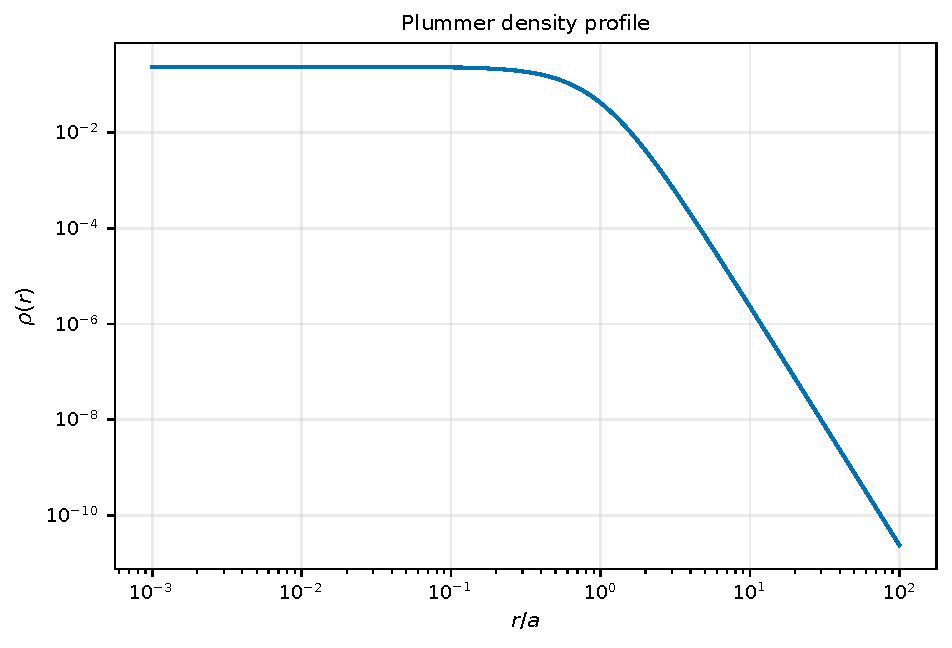
\includegraphics[width=\linewidth]{ch01_plummer_density.pdf}
\end{minipage}\hfill
\begin{minipage}[t]{0.47\linewidth}
\centering
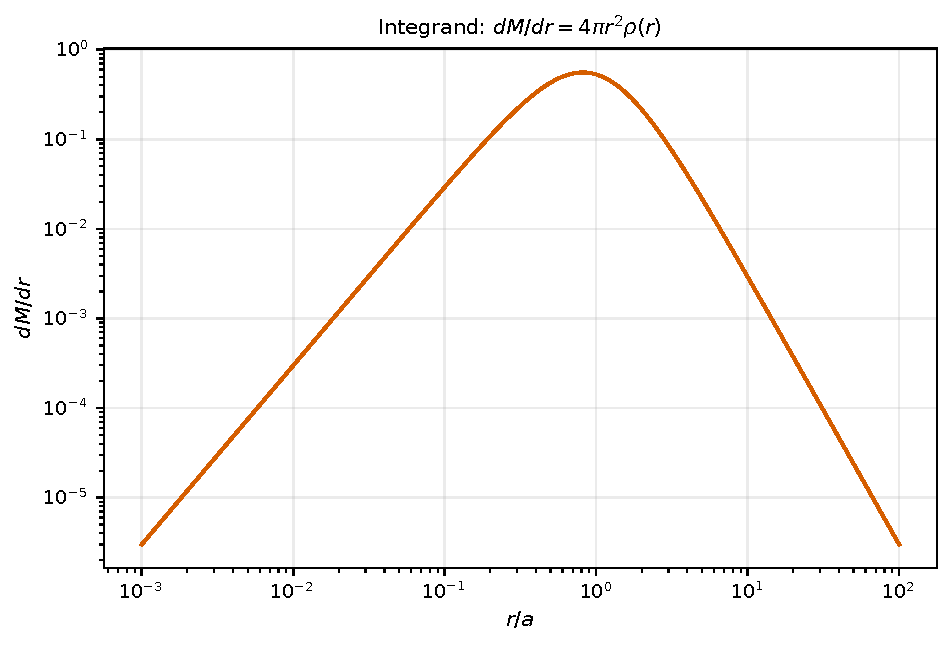
\includegraphics[width=\linewidth]{ch01_mass_integrand.pdf}
\end{minipage}
\caption{Plummer 密度分布の密度（左）と、内包質量の被積分関数 $dM/dr=4\pi r^2\rho$（右）。縦軸はそれぞれ $M/a^3$、$M/a$ を単位としている。密度は中心で最大であるが、同じ厚さの球殻の体積は $r^2$ に比例するため、$dM/dr$ は中心で0になる。}
\label{fig:ch1-plummer-integrand}
\end{figure}

\subsection{解析的な内包質量}

式\eqref{eq:ch1-plummer-density}のPlummer 密度分布では式\eqref{eq:ch1-enclosed-mass}を解析的に積分できる。
無次元半径
\begin{equation}
 x\equiv \frac{r}{a}
\label{eq:ch1-x-def}
\end{equation}
を導入する。積分変数を $u=r'/a$ に取り替えると、$r'=au$、$dr'=a\,du$ であり、積分の上端は $u=x$ になるので、
\begin{align}
 M(<r) =4\pi\int_0^r \rho(r')r'^2\,dr' =3M\int_0^x \frac{u^2}{(1+u^2)^{5/2}}\,du.
\label{eq:ch1-plummer-mass-int}
\end{align}
実際、
\begin{equation}
 \frac{d}{du}\left[\frac{u^3}{(1+u^2)^{3/2}}\right]
 =\frac{3u^2}{(1+u^2)^{5/2}}
\end{equation}
なので、この積分は解析的に計算できる。したがって、
\begin{equation}
 \boxed{
 M(<r)
 =M\frac{x^3}{(1+x^2)^{3/2}}
 =M\frac{(r/a)^3}{\left[1+(r/a)^2\right]^{3/2}}
 }
\label{eq:ch1-plummer-mass-exact}
\end{equation}
を得る。
$r\rightarrow\infty$ では $M(<r)\rightarrow M$ となり、$M$ が全質量であることも確認できる。
本章では式\eqref{eq:ch1-plummer-mass-exact}を「正解」として使い、数値積分の精度を検証する。

以後、本章では半径を $a$、質量を $M$ で規格化し、$r/a$ と $M(<r)/M$ を用いて結果を表す。
Notebook 1 では、この規格化を $M=a=1$ として実装する。
これは質量と長さの単位を選んで無次元量を扱っているだけであり、両者を同じ物理量とみなすことを意味しない。

\section{数値積分の考え方}
\label{sec:ch1-quadrature-basics}

数値積分の積分公式を導くため、ここでは $x$ を無次元半径に限らず一般の積分変数として用い、定積分
\begin{equation}
 I=\int_{x_0}^{x_N} f(x)\,dx
\label{eq:ch1-general-integral}
\end{equation}
を考える。
区間 $[x_0,x_N]$ を $N$ 個の小区間に等分し、格子点を
\begin{equation}
 x_i=x_0+ih,
 \qquad
 h=\frac{x_N-x_0}{N}
\label{eq:ch1-uniform-grid}
\end{equation}
とする。ここで $h$ は隣り合う格子点の間隔であり、\textbf{格子幅（grid spacing）}と呼ぶ。
$N$ は区間数であり、両端を含む格子点数は $N+1$ である。
この分割によって定積分$I$は
\begin{equation}
 I=\sum_{i=0}^{N-1}
 \int_{x_i}^{x_{i+1}} f(x)\,dx
\label{eq:ch1-split-integral}
\end{equation}
と書けることになる。

数値積分では、各小区間で $f(x)$ を簡単な関数で近似して積分する。
例えば一定値で近似すれば長方形、1次関数なら台形、2次関数なら Simpson 則が得られる。

\section{基本的な数値積分公式}
\label{sec:ch1-basic-rules}

図\ref{fig:ch1-quadrature-geometry}に、4種類の積分公式の幾何学的な考え方を示す\footnote{
ここでは4つの積分公式を紹介するが、格子点上の値を積分する実際の計算では台形則がよく使われる。
左長方形則は台形則と同じ格子点の値を使うにもかかわらず、誤差の減り方が遅い（\S\ref{sec:ch1-convergence}）。
中点則は区間の中点での値を必要とするため、格子点の値しかないデータにはそのまま使えない。
ただし、セル中心に値を置く計算や、端点で被積分関数が発散する積分では中点則が適している。
台形則は隣り合う2点の値だけで計算でき、不等間隔の格子にも使え、
区間ごとの面積を順に足すだけで累積積分が得られる（\S\ref{sec:ch1-cumulative}）。
Simpson 則は被積分関数が滑らかなときに誤差が速く減少するが、区間を2つずつ組にする必要があり、
折れ曲がりや雑音を含むデータでは、その利点は小さくなる。
格子法の流体計算で用いる有限体積法では、密度などのセル平均値を未知数とする。
一次元の Cartesian 座標で、幅 $h$ のセルを中心のまわりに対称に取ると、滑らかな関数のセル平均とセル中心の値との差は $O(h^2)$ となる。
この関係は、中点則の誤差と同じように Taylor 展開から説明できる\cite{matsumoto}。}。
以下では、各公式が被積分関数をどのように近似するかと、その実装方法を順に見ていく。
それぞれの方法で誤差がどの速さで減少するかは、後の収束試験で数値的に調べる。

\begin{figure}[!htbp]
\centering
\begin{minipage}[t]{0.47\linewidth}
\centering
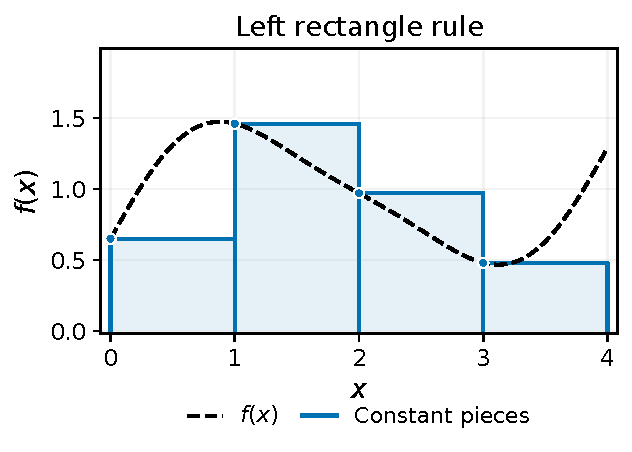
\includegraphics[width=\linewidth]{ch01_left_rule.pdf}\\[-1mm]
{\small (a) Left rectangle}
\end{minipage}\hfill
\begin{minipage}[t]{0.47\linewidth}
\centering
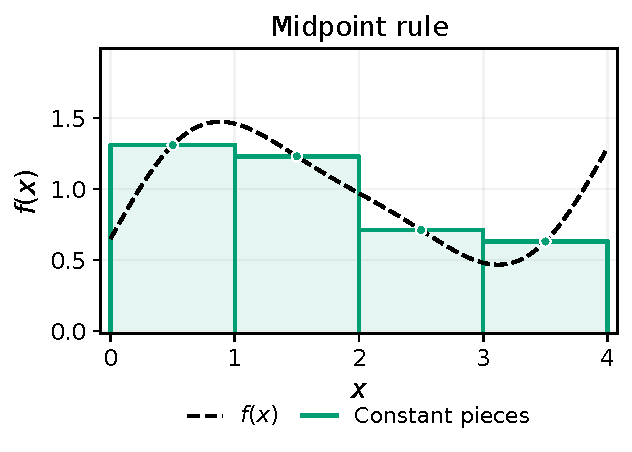
\includegraphics[width=\linewidth]{ch01_midpoint_rule.pdf}\\[-1mm]
{\small (b) Midpoint}
\end{minipage}

\vspace{2mm}
\begin{minipage}[t]{0.47\linewidth}
\centering
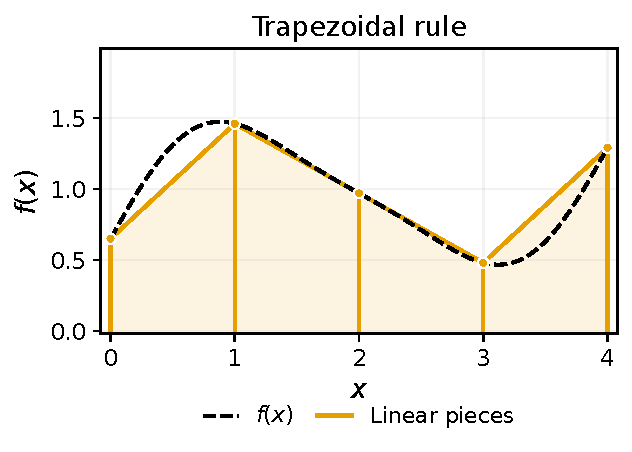
\includegraphics[width=\linewidth]{ch01_trapezoid_rule.pdf}\\[-1mm]
{\small (c) Trapezoidal}
\end{minipage}\hfill
\begin{minipage}[t]{0.47\linewidth}
\centering
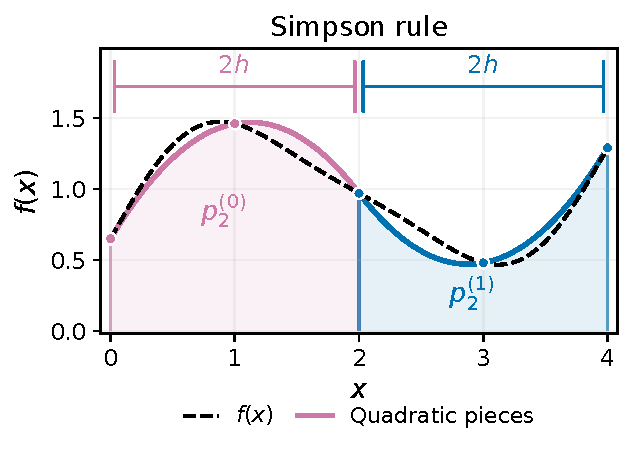
\includegraphics[width=\linewidth]{ch01_simpson_rule.pdf}\\[-1mm]
{\small (d) Simpson}
\end{minipage}
\caption{数値積分公式の幾何学的な意味。黒破線は全パネルで共通の被積分関数 $f(x)$、色付き実線は各方法の近似である。Simpson 則では幅 $2h$ の各区間で、3個の評価点を通る別々の二次多項式 $p_2^{(0)},p_2^{(1)}$ を積分する。色付きの面積が積分の近似値に対応する。}
\label{fig:ch1-quadrature-geometry}
\end{figure}

\subsection{左長方形則（left-rectangle rule）}

小区間 $[x_i,x_{i+1}]$ で $f(x)$ を左端の値 $f_i\equiv f(x_i)$ で一定と近似すると、
\begin{equation}
 \int_{x_i}^{x_{i+1}}f(x)\,dx
 \simeq hf_i
\label{eq:ch1-left-local}
\end{equation}
である。この近似では、各小区間の左端 $x_i=x_0+ih$ だけで関数を評価していることになる。
全区間を足すと、左長方形則は次のように書ける。
\begin{equation}
 \boxed{
 I_{\rm left}
 =h\sum_{i=0}^{N-1}f_i
 }
\label{eq:ch1-left-rule}
\end{equation}
Python では Listing 1.1 のように書ける。
\begin{listingbox}{1.1　左長方形則}
\begin{Verbatim}[fontsize=\small]
import numpy as np
def left_rule(func, x0, xN, N):
    h = (xN - x0) / N
    x = x0 + np.arange(N) * h
    return h * np.sum(func(x))
\end{Verbatim}
\end{listingbox}



\subsection{中点則（midpoint rule）}

小区間 $[x_i,x_{i+1}]$ で $f(x)$ を中点
\begin{equation}
 x_{i+1/2}=x_i+\frac{h}{2}
\label{eq:ch1-midpoint-def}
\end{equation}
での関数値を使えば、
\begin{equation}
 \boxed{
 I_{\rm mid}
 =h\sum_{i=0}^{N-1}f(x_{i+1/2})
 }
\label{eq:ch1-midpoint-rule}
\end{equation}
を得る。

中点 $x_{i+1/2}=x_i+h/2$ は、格子番号 $i$ に $1/2$ を加えて作れる。
式\eqref{eq:ch1-midpoint-rule}の実装が Listing 1.2 である。
\begin{listingbox}{1.2　中点則}
\begin{Verbatim}[fontsize=\small]
def midpoint_rule(func, x0, xN, N):
    h = (xN - x0) / N
    x_mid = x0 + (np.arange(N) + 0.5) * h
    return h * np.sum(func(x_mid))
\end{Verbatim}
\end{listingbox}


\subsection{台形則（trapezoidal rule）}

台形則では、小区間内の $f(x)$ を両端 $(x_i,f_i)$ と $(x_{i+1},f_{i+1})$ を結ぶ直線で近似する。
直線補間（linear interpolation）は
\begin{equation}
 f(x)
 \simeq f_i
 +\frac{f_{i+1}-f_i}{h}(x-x_i)
\label{eq:ch1-linear-interpolation}
\end{equation}
である。
これを $x_i$ から $x_{i+1}$ まで積分すると、
\begin{align}
 \int_{x_i}^{x_{i+1}}f(x)\,dx
 &\simeq
 \int_{x_i}^{x_{i+1}}
 \left[
 f_i+\frac{f_{i+1}-f_i}{h}(x-x_i)
 \right]dx \\
 &=\frac{h}{2}(f_i+f_{i+1}).
\label{eq:ch1-trapezoid-panel}
\end{align}
これが台形の面積そのものである。
全区間を足すと内部格子点は2回ずつ現れるため、
\begin{equation}
 \boxed{
 I_{\rm trap}
 =h\left[
 \frac{1}{2}f_0
 +\sum_{i=1}^{N-1}f_i
 +\frac{1}{2}f_N
 \right]
 }
\label{eq:ch1-trapezoid-rule}
\end{equation}
を得る。

式\eqref{eq:ch1-trapezoid-rule}の各項をそのまま Python に対応させると、Listing 1.3 のように書ける。
\begin{listingbox}{1.3　台形則}
\begin{Verbatim}[fontsize=\small]
def trapezoid_rule(func, x0, xN, N):
    h = (xN - x0) / N
    x = np.linspace(x0, xN, N + 1)
    y = func(x)

    return h * (0.5 * y[0] + np.sum(y[1:-1]) + 0.5 * y[-1])
\end{Verbatim}
\end{listingbox}
左長方形則と中点則では各小区間の代表点 $N$ 個を使ったが、台形則では両端を含む $N+1$ 個の格子点を使う。この実装では、それらを \texttt{np.linspace(x0, xN, N + 1)} で作っている。
$f_0$ と $f_N$ が \texttt{y[0]}, \texttt{y[-1]} に、
内部点の和 $\sum_{i=1}^{N-1}f_i$ が \texttt{np.sum(y[1:-1])} に対応する。


\subsection{Simpson 則（Simpson's rule）}
Simpson 則では、隣り合う2つの小区間を1組として扱う。まず1組 $[x_i,x_{i+2}]$ を取り出し、等間隔の3点
\begin{equation}
 x_i,\qquad x_{i+1}=x_i+h,\qquad x_{i+2}=x_i+2h
\label{eq:ch1-simpson-nodes}
\end{equation}
における関数値を $f_i,f_{i+1},f_{i+2}$ とする。
この3点を通る2次多項式で $f(x)$ を近似し、その多項式を積分する。

計算を簡単にするため、区間の中央 $x_{i+1}$ を原点とする無次元変数
\begin{equation}
 t=\frac{x-x_{i+1}}{h}
\label{eq:ch1-simpson-t}
\end{equation}
を導入する。このとき、3点は $t=-1,0,1$ に対応する。
2次多項式を
\begin{equation}
 p_2(t)=At^2+Bt+C
\end{equation}
とおく。3点を通る条件は
\begin{align}
 p_2(-1)&=A-B+C=f_i,\\
 p_2(0)&=C=f_{i+1},\\
 p_2(1)&=A+B+C=f_{i+2}
\end{align}
である。これらを解くと、
\begin{equation}
 A=\frac{f_i-2f_{i+1}+f_{i+2}}{2},\qquad
 B=\frac{f_{i+2}-f_i}{2},\qquad
 C=f_{i+1}
\end{equation}
を得る。

$dx=h\,dt$ なので、
\begin{align}
 \int_{x_i}^{x_{i+2}}f(x)\,dx
 &\simeq h\int_{-1}^{1}p_2(t)\,dt
 \label{eq:ch1-simpson-integral-p2}\\
 &=h\int_{-1}^{1}(At^2+Bt+C)\,dt \notag\\
 &=h\left(\frac{2A}{3}+2C\right) \notag\\
 &=\frac{h}{3}(f_i+4f_{i+1}+f_{i+2})
 \label{eq:ch1-simpson-panel}
\end{align}
を得る。
これが1組に対する Simpson の1/3公式である\cite{kouya2021}。

次に、積分区間全体を幅 $h$ の $N$ 個の小区間に分割する。
Simpson 則は2つの小区間を1組として適用するため、$N$ は偶数とする。
例えば、$N=4$ の場合を考える。
最初の組 $[x_0,x_2]$ と次の組 $[x_2,x_4]$ にSimpson 則を適用して足し合わせると、
\begin{align}
 I_{\rm Simpson}
 &=
 \frac{h}{3}(f_0+4f_1+f_2)
 +\frac{h}{3}(f_2+4f_3+f_4)\\
 &=
 \frac{h}{3}(f_0+4f_1+2f_2+4f_3+f_4)
\end{align}
となる。
ここで、$f_2$ は両方の組に含まれるため、係数が2になる。
同様に、$N$ が一般の偶数の場合には、積分区間の両端の係数が1、奇数番号の点の係数が4、
両端を除く偶数番号の点の係数が2となる。したがって、
\begin{equation}
 \boxed{
 I_{\rm Simpson}
 =\frac{h}{3}\left[
 f_0+f_N
 +4\sum_{j=1}^{N/2}f_{2j-1}
 +2\sum_{j=1}^{N/2-1}f_{2j}
 \right]
 }
\label{eq:ch1-composite-simpson}
\end{equation}
を得る。

この公式では、奇数番号と偶数番号の内部点を別々に足す必要がある。
NumPy のスライスを使うと、Listing 1.4 のように数式の構造をほぼそのまま表現できる。
\begin{listingbox}{1.4　Simpson 則}
\begin{Verbatim}[fontsize=\small]
def simpson_rule(func, x0, xN, N):
    if N % 2 != 0:
        raise ValueError("Simpson 則では N を偶数にしてください。")

    h = (xN - x0) / N
    x = np.linspace(x0, xN, N + 1)
    y = func(x)

    odd_sum = np.sum(y[1:-1:2])
    even_sum = np.sum(y[2:-1:2])

    return h / 3.0 * (y[0] + y[-1] + 4.0 * odd_sum + 2.0 * even_sum)
\end{Verbatim}
\end{listingbox}

\texttt{y[1:-1:2]} は $y_1,y_3,y_5,\ldots$、
\texttt{y[2:-1:2]} は $y_2,y_4,y_6,\ldots$ を取り出す。
したがって、それぞれ式\eqref{eq:ch1-composite-simpson}の奇数番号の和と偶数番号の和に対応する。


\section{Plummer 球による4つの積分法の比較}
\label{sec:ch1-compare-rules}

Plummer 球について、半径 $r=a$ までの内包質量を求める。$x=r/a$ を用いると、
式\eqref{eq:ch1-plummer-mass-int}より、比較する積分は
\begin{equation}
 I\equiv\frac{M(<a)}{M}=\int_0^1\frac{3x^2}{(1+x^2)^{5/2}}\,dx
\label{eq:ch1-plummer-test-integral}
\end{equation}
である。すなわち、$f(x)=3x^2/(1+x^2)^{5/2}$ に前節で導いた4つの積分公式を適用する。
この $f(x)$ は、式\eqref{eq:ch1-mass-integrand}の被積分関数 $f_M(r)=dM/dr$ を $M/a$ で割り、$r=ax$ としたものである。Notebook 1 では $M=a=1$ とするため、\texttt{dMdr\_plummer} の返す値がそのまま $f(x)$ に対応する。

数値積分の精度を評価するために、格子幅 $h$ で求めた数値積分値を $I_h$ とし、解析値 $I$ との差の大きさ
\begin{equation}
 \epsilon(h)\equiv |I_h-I|
\label{eq:ch1-absolute-error}
\end{equation}
を\textbf{絶対誤差（absolute error）}と定義する。これは、全質量 $M$ で規格化した内包質量の誤差である。
なお、ここでは $r=a$ を評価点とし、解析値
\begin{equation}
 I=\frac{M(<a)}{M}=\frac{1}{2\sqrt{2}}
 \simeq \choneMExactA
\label{eq:ch1-mass-at-a}
\end{equation}
を比較基準とする。

\begin{notebookblock}{1｜4つの積分法の比較}
$M=a=1$、$N=40$ として、4つの積分法を同じ条件で比較する。数値積分値と解析値との差から絶対誤差を計算し、その結果を同じセルの出力として表示する。

{\sffamily\small\color{graytext}対応セル（計算部分）}
\begin{Verbatim}[xleftmargin=2mm,fontsize=\small,frame=single,framesep=1.8mm,framerule=0.35pt,rulecolor=\color{listingframe},fillcolor=\color{listingbg}]
# 積分区間を 0 <= r <= a とし、区間数を N=40 にする
r_eval = 1.0 * a
N = 40

# 被積分関数 dM/dr = 4 pi r^2 rho(r)
func = lambda r: dMdr_plummer(r, M, a)

# 同じ条件で4つの数値積分法を適用する
m_left = left_rule(func, 0.0, r_eval, N)
m_mid = midpoint_rule(func, 0.0, r_eval, N)
m_trap = trapezoid_rule(func, 0.0, r_eval, N)
m_simp = simpson_rule(func, 0.0, r_eval, N)

# 数値積分値と比較する解析値
m_exact_eval = mass_plummer_exact(r_eval, M, a)

print(f"解析値     : {m_exact_eval:.12f}")
print(f"左長方形則  : {m_left:.12f}   誤差 = {abs(m_left - m_exact_eval):.3e}")
print(f"中点則     : {m_mid:.12f}   誤差 = {abs(m_mid - m_exact_eval):.3e}")
print(f"台形則     : {m_trap:.12f}   誤差 = {abs(m_trap - m_exact_eval):.3e}")
print(f"Simpson 則 : {m_simp:.12f}   誤差 = {abs(m_simp - m_exact_eval):.3e}")
\end{Verbatim}

{\sffamily\small\color{graytext}実行結果}
\begin{Verbatim}[numbers=none,fontsize=\small]
解析値                : 0.353553390593
左長方形則            : 0.346910451143   誤差 = 6.643e-03
中点則                : 0.353560298293   誤差 = 6.908e-06
台形則                : 0.353539577216   誤差 = 1.381e-05
Simpson 則            : 0.353553401385   誤差 = 1.079e-08
\end{Verbatim}
\end{notebookblock}

この結果から、$N=40$ では Simpson 則の誤差が最も小さいことがわかる。
しかし、この1つの格子だけでは、格子を細かくしたときに誤差がどのように減るかは分からない。
そこで次に、格子幅と絶対誤差 $\epsilon(h)$の関係を調べる収束試験を行う。

\section{収束次数の測定}
\label{sec:ch1-convergence}

\subsection{誤差の $h$ 依存性}

前節では、$N=40$ の1つの格子で4つの積分法の誤差を比較した。
次に、格子幅 $h$ を小さくしたときに、絶対誤差 $\epsilon(h)$ がどの速さで減少するかを調べる。
多くの数値計算法では、格子を十分に細かくすると、誤差は格子幅 $h$ のべき乗に従って規則的に減少する。
この誤差の減少の速さを表す量を\textbf{収束次数}という。

\begin{definitionbox}{収束次数}
十分小さい格子幅 $h$ に対して、誤差が
\begin{equation}
 \epsilon(h)\simeq C h^p
\label{eq:ch1-error-model}
\end{equation}
と振る舞うとき、指数 $p>0$ をその数値計算法の\textbf{収束次数（order of convergence）}と呼ぶ。
ここで $C>0$ は $h$ に依存しない定数である。
\end{definitionbox}

収束次数が $p$ の方法を、\textbf{$p$ 次精度}の方法と呼ぶ。
例えば $p=2$ なら、格子幅を半分にすると誤差はおよそ $1/4$ になる。
$p=4$ なら、およそ $1/16$ になる。
したがって、収束次数が大きい方法ほど、格子を細かくしたときに誤差が速く減少する。

\begin{cautionblock}{収束次数と誤差の大きさは同じではない}
式\eqref{eq:ch1-error-model}では、収束次数 $p$ は格子幅を小さくしたときに誤差がどの速さで減るかを表し、係数 $C$ は誤差の大きさに関係する。
したがって、同じ収束次数をもつ方法でも、同じ $h$ での誤差が同じとは限らない。
また、有限の $h$ では、収束次数が高い方法が必ず最小の誤差を与えるとは限らない。
\end{cautionblock}

\subsection{数値実験による収束次数の測定}

それでは、Plummer 球の内包質量を用いて、実際に収束次数を測ってみる。
収束次数を数値的に測定するには、式\eqref{eq:ch1-error-model}の対数を取り、
\begin{equation}
 \log\epsilon
 =p\log h+\log C
\label{eq:ch1-log-error}
\end{equation}
とする。
したがって、$\log\epsilon$ を $\log h$ に対してプロットすると、式\eqref{eq:ch1-error-model}が成り立つ範囲では点列はほぼ直線上に並び、その傾きが収束次数 $p$ となる。
対数の底を変えても傾き $p$ は変わらない。Notebook 1 では、\texttt{np.log} と \texttt{np.polyfit} を用いて複数の格子幅の点を直線で近似し、その傾きから $p$ を求める。

そこで、複数の格子幅で同じ積分を計算し、解析値との差から得た絶対誤差を用いて収束次数を測定する。
どの積分公式で $p$ がどの程度になるかを、まず数値実験から確かめてみる。

\begin{notebookblock}{1｜収束試験}
左長方形則・中点則・台形則・Simpson 則について、$N=10,20,40,80,160,320$ と格子を細かくする。各方法について $\log\epsilon$ と $\log h$ を直線で近似し、その傾きから収束次数 $p$ を求める。
そのために、ここでは NumPy の \texttt{np.polyfit(x, y, 1)} を用いる。
この関数は、データ $(x,y)$ を直線 $y=ax+b$ で最小二乗近似し、傾き $a$ と切片 $b$ をこの順に返す。
したがって、末尾の \texttt{[0]} で傾き、すなわち収束次数 $p$ を取り出す。

{\sffamily\small\color{graytext}対応セル（計算部分）}
\begin{Verbatim}[xleftmargin=2mm,fontsize=\small,frame=single,framesep=1.8mm,framerule=0.35pt,rulecolor=\color{listingframe},fillcolor=\color{listingbg}]
# 区間数 N を2倍ずつ増やして格子幅を小さくする
N_values = np.array([10, 20, 40, 80, 160, 320])
h_values = r_eval / N_values

# 4つの積分法を同じ形で呼び出せるようにまとめる
methods = {
    "Left rectangle": lambda N: left_rule(func, 0.0, r_eval, N),
    "Midpoint": lambda N: midpoint_rule(func, 0.0, r_eval, N),
    "Trapezoidal": lambda N: trapezoid_rule(func, 0.0, r_eval, N),
    "Simpson": lambda N: simpson_rule(func, 0.0, r_eval, N),
}

errors = {}
orders = {}
for name, method in methods.items():
    # 各 N で解析値との差を絶対誤差として測る
    err = np.array([abs(method(int(N)) - m_exact_eval) for N in N_values])
    errors[name] = err

    # log(error)-log(h) の傾きから収束次数 p を求める
    orders[name] = np.polyfit(np.log(h_values), np.log(err), 1)[0]

method_names_ja = {
    "Left rectangle": "左長方形則",
    "Midpoint": "中点則",
    "Trapezoidal": "台形則",
    "Simpson": "Simpson 則",
}

for name in methods:
    print(f"{method_names_ja[name]:10s}: 測定した収束次数 = {orders[name]:.3f}")
\end{Verbatim}

{\sffamily\small\color{graytext}実行結果}
\begin{Verbatim}[numbers=none,fontsize=\small]
左長方形則     : 測定した収束次数 = 1.002
中点則         : 測定した収束次数 = 2.001
台形則         : 測定した収束次数 = 2.001
Simpson 則     : 測定した収束次数 = 4.001
\end{Verbatim}
\end{notebookblock}

この結果から、左長方形則はほぼ1次、中点則と台形則はほぼ2次、Simpson 則はほぼ4次で収束していることがわかる。
また、誤差と格子幅の関係を図\ref{fig:ch1-convergence}に示す。各方法の点列は両対数表示でほぼ直線となり、その傾きがそれぞれの収束次数に対応している。

このような\textbf{格子収束試験（grid-convergence test）}は、数値計算法の収束次数を実際の計算から調べる基本的な検証方法である。ただし、格子を極端に細かくすると、誤差がこのべき則から外れる場合がある。その主な原因の一つが、次節で扱う浮動小数点演算の丸め誤差である。

\begin{figure}[!htbp]
\centering
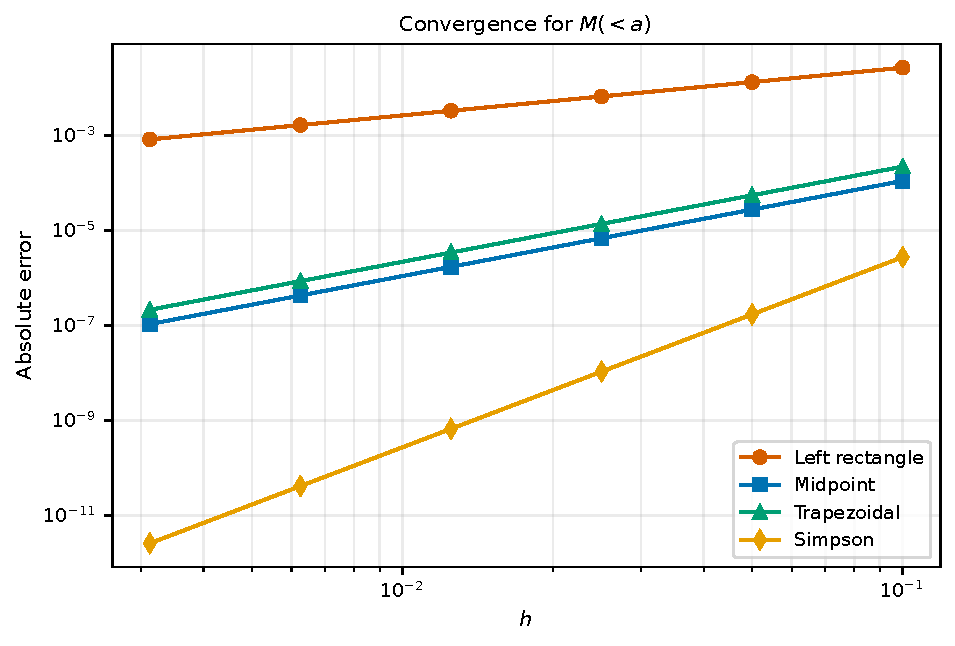
\includegraphics[width=0.6\linewidth]{ch01_convergence.pdf}
\caption{$M(<a)/M$ の絶対誤差と格子幅 $h$ の関係。両対数表示での傾きが収束次数 $p$ である。ここで $h$ は無次元半径 $x=r/a$ に対する格子幅であり、$h=1/N$ である。}
\label{fig:ch1-convergence}
\end{figure}



\begin{topicblock}{Taylor 展開から収束次数を理解する}
ここまでの収束試験では、数値実験から左長方形則、中点則、台形則、Simpson 則の収束次数を測定した。
ここでは中点則を例に、なぜ局所的な近似誤差から積分全体の収束次数が決まるのかを見る。
この補足は、以後の節を理解するための必須事項ではない。

以下で $O(h^q)$ は、$h\rightarrow0$ のとき、その項の大きさが $h^q$ の定数倍以下に抑えられることを表す。
1区間で生じる誤差を\textbf{局所打ち切り誤差}、積分区間全体で得られる誤差を\textbf{大域誤差}と呼ぶ。

中点則を区間 $[x_i,x_{i+1}]$ に適用する。
区間幅を $h=x_{i+1}-x_i$、中点を
\begin{equation}
 x_{i+1/2}=\frac{x_i+x_{i+1}}{2}
\end{equation}
とする。
中点からのずれを $\xi=x-x_{i+1/2}$ とおけば、積分範囲は
$-h/2\le\xi\le h/2$ となる。
中点のまわりで Taylor 展開すると、
\begin{equation}
 f(x_{i+1/2}+\xi)
 =
 f_{i+1/2}
 +\xi f'_{i+1/2}
 +\frac{\xi^2}{2}f''_{i+1/2}
 +\frac{\xi^3}{6}f'''_{i+1/2}
 +O(\xi^4)
\end{equation}
である。
これを $-h/2$ から $h/2$ まで積分する。
対称な区間では $\xi$ と $\xi^3$ のような奇数次の項の積分が0になるので、
\begin{align}
 \int_{x_i}^{x_{i+1}}f(x)\,dx
 &=
 \int_{-h/2}^{h/2}f(x_{i+1/2}+\xi)\,d\xi \notag\\
 &=
 h f_{i+1/2}
 +\frac{h^3}{24}f''_{i+1/2}
 +O(h^5)
\label{eq:ch1-midpoint-error-advanced}
\end{align}
を得る。

中点則は右辺の最初の項 $h f_{i+1/2}$ だけを使う。
したがって、1区間での局所打ち切り誤差は
\begin{equation}
 E_i
 =
 \frac{h^3}{24}f''_{i+1/2}
 +O(h^5)
 =
 O(h^3)
\end{equation}
である。

次に、積分区間全体 $[a,b]$ を考える。
区間数は
\begin{equation}
 N=\frac{b-a}{h}\propto h^{-1}
\end{equation}
である。
$f''$ が積分区間で有界なら、各区間の局所打ち切り誤差は一様に $O(h^3)$ なので、
それらを $N$ 区間にわたって合わせた大域誤差は
\begin{equation}
 E
 =\sum_{i=0}^{N-1}E_i
 =O(Nh^3)
 =O(h^2)
\end{equation}
となる。
したがって、中点則は\textbf{2次精度}である。

他の積分公式でも考え方は同じである。
局所打ち切り誤差が $O(h^{p+1})$ なら、固定した積分区間では区間数が
$O(h^{-1})$ であるため、大域誤差は $O(h^p)$ となる。本章で用いた4つの公式では以下のようになる。
なお、Simpson 則では2区間1組を単位として局所誤差を数えるが、
組の数も $O(h^{-1})$ なので同じ考え方で4次精度が得られる。
\begin{center}
\begin{tabular}{lcc}
\toprule
方法 & 局所打ち切り誤差 & 大域誤差 \\
\midrule
左長方形則 & $O(h^2)$ & $O(h)$ \\
中点則 & $O(h^3)$ & $O(h^2)$ \\
台形則 & $O(h^3)$ & $O(h^2)$ \\
Simpson 則 & $O(h^5)$ & $O(h^4)$ \\
\bottomrule
\end{tabular}
\end{center}

この結果は、Notebook 1 の収束試験で測定した
$p\simeq1,2,2,4$ と一致する。
より一般的な積分則の誤差評価については杉浦 第3章\cite{sugiura2009}を、
Newton--Cotes 型積分公式の導出と実装については幸谷 第12章\cite{kouya2021}を参照されたい。
\end{topicblock}

\section{離散化誤差と丸め誤差}
\label{sec:ch1-roundoff}

前節の収束試験では、格子幅 $h$ を小さくすると、数値積分の誤差が $h^p$ に従って減少することを確認した。
数値計算では、このような数値公式による近似だけでなく、計算機が有限桁の数を扱うことによっても誤差が生じる。
本節では、これらに対応する\textbf{離散化誤差}と\textbf{丸め誤差}について考える。

\subsection{離散化誤差（discretization error）}

数値計算では、連続な問題をそのまま計算機で扱うのではなく、有限個の格子点や時間刻みを用いた離散的な問題に置き換える。
本章の数値積分では、積分区間を有限個の小区間に分け、それぞれの区間で被積分関数を簡単な関数で近似した。
このような離散化によって、数値積分値には厳密な積分値との差が生じる。
この差を\textbf{離散化誤差（discretization error）}という。

離散化によって生じる誤差は、「1回の近似でどれだけずれるか」と「計算全体の結果がどれだけずれるか」という2つの観点から見ることができる。
数値積分では、各小区間で近似を行うたびに誤差が生じ、それらを全区間に適用した最終的な積分値にも誤差が残る。
この2つの見方に対応するのが、局所打ち切り誤差と大域誤差である。

\begin{definitionbox}{局所打ち切り誤差と大域誤差}
微分、積分、時間発展などの連続な関係を有限の近似式へ置き換えたときに生じるずれを
\textbf{打ち切り誤差（truncation error）}という。
本書では、1つの小区間、1ステップ、または1格子点で評価したものを
\textbf{局所打ち切り誤差（local truncation error）}と呼ぶ。

一方、離散公式を計算全体に適用して得られた数値結果と厳密な結果との差を
\textbf{大域誤差（global error）}という。
本章の数値積分では、丸め誤差などを無視できる場合、大域誤差は各区間の局所的な打ち切り誤差を積分範囲全体で合わせた結果として現れる。
時間発展を伴う問題では、局所的な誤差の伝播や増幅も重要になる。
\end{definitionbox}

前節の収束試験で測定した収束次数 $p$ は、この大域誤差が格子幅 $h$ に対してどの速さで減少するかを表している。
本章の例では、左長方形則の誤差はおよそ $h$、中点則と台形則では $h^2$、Simpson 則では $h^4$ に比例して減少した。
離散化誤差だけを考えるなら、格子幅 $h$ を小さくするほど数値積分値は解析値に近づく。

\subsection{丸め誤差（round-off error）}

実際の計算機では、実数を無限の精度で表すことはできない。
数値計算では、実数を有限桁の\textbf{浮動小数点数（floating-point number）}で近似して扱う。
浮動小数点数とは、例えば $1.23\times 10^4$ のように、数を有効数字と指数に分けて表す方法である。
計算機では通常、2進数を用いて数を表すが、表現できる有効桁数には限りがある。
そのため、演算結果が表現可能な数に一致しない場合には、近くの値へ丸められる。
このように、有限桁の浮動小数点数で数値を表し、演算結果を丸めることによって生じる誤差を
\textbf{丸め誤差（round-off error）}という。

浮動小数点数の精度を表す目安の一つが、\textbf{機械イプシロン（machine epsilon）}である。
機械イプシロン $\epsilon_{\rm mach}$ は、1と、それより大きい最も近い浮動小数点数との差として定義される。
つまり、1付近でどれほど小さな数の差を区別できるかを表している。
Notebook 1 で用いる倍精度浮動小数点数（64ビット）では、
\begin{equation}
 \epsilon_{\rm mach}\simeq \choneMachineEps
\label{eq:ch1-machine-eps}
\end{equation}
である\cite{kouya2021}。
ただし、機械イプシロンは計算結果全体の誤差を表すものではない。
丸め誤差は演算を繰り返すことで蓄積する場合がある。
また、近い値どうしを引くと、もとの数値に含まれる小さな誤差が計算結果に大きく影響することがある。

一般に、格子を細かくすると離散化誤差は小さくなる。
しかし、離散化誤差が十分に小さくなると、丸め誤差の影響を無視できなくなる場合がある。
そのため、格子を細かくしても計算精度が上がり続けるとは限らない。
Simpson 則では離散化誤差がおよそ $h^4$ に比例して速く減少するため、この変化を確認しやすい。

\begin{notebookblock}{1｜Simpson 則と丸め誤差}
$N\sim10^3$--$10^4$ 以上まで増やし、離散化誤差が十分小さくなった後に丸め誤差の影響が現れる様子を確認する。

{\sffamily\small\color{graytext}対応セル（計算部分）}
\begin{Verbatim}[xleftmargin=2mm,fontsize=\small,frame=single,framesep=1.8mm,framerule=0.35pt,rulecolor=\color{listingframe},fillcolor=\color{listingbg}]
# Simpson 則で、さらに細かい格子まで調べる
N_large = np.array([320, 640, 1280, 2560,
                    5120, 10240, 20480])
err_large = []

for N_i in N_large:
    # 各 N で Simpson 則を適用し、解析値との誤差を保存する
    val = simpson_rule(func, 0.0, r_eval, int(N_i))
    err_large.append(abs(val - m_exact_eval))

# 倍精度浮動小数点数の機械イプシロン
machine_eps = np.finfo(float).eps
\end{Verbatim}
\end{notebookblock}

図\ref{fig:ch1-roundoff}に示すように、この計算では区間数を増やすと、
最初は $h^4$ に従って誤差が減少する。
しかし、誤差が $10^{-15}$--$10^{-16}$ 程度まで小さくなると
丸め誤差の影響が現れ、この関係から外れる。
この領域では、格子をさらに細かくしても精度は系統的には向上しない。

\begin{figure}[!htbp]
\centering
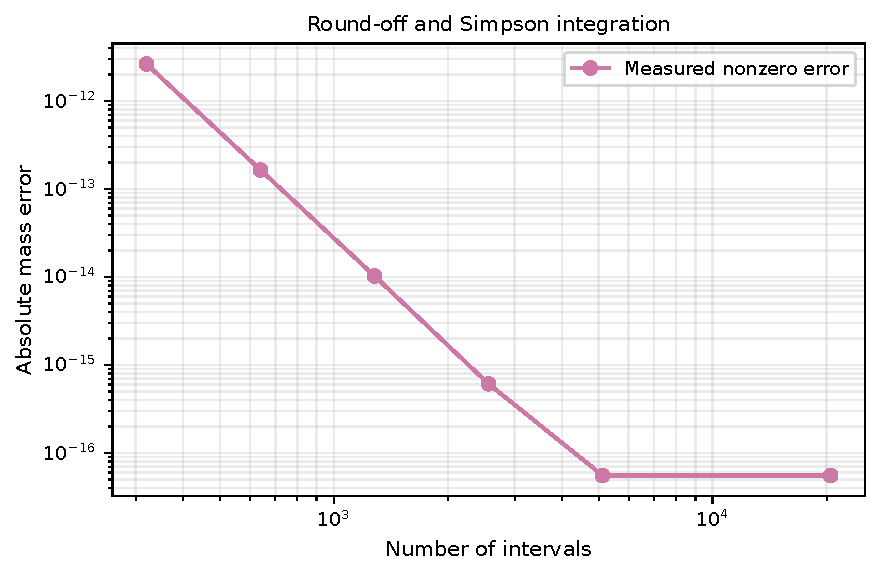
\includegraphics[width=0.68\linewidth]{ch01_roundoff.pdf}
\caption{Simpson 則の区間数 $N$ を増やしたときの、$M(<a)/M$ の絶対誤差。
離散化誤差が十分小さくなると、倍精度浮動小数点数の丸め誤差の影響が見えてくる。}
\label{fig:ch1-roundoff}
\end{figure}


\section{累積積分による内包質量プロファイル}
\label{sec:ch1-cumulative}

これまでは固定した半径 $r=a$ までの1つの定積分を比較した。次に、すべての格子点 $r_i$ について $M(<r_i)$ を求める。
しかし、各半径について0から積分をやり直すと、同じ区間の寄与を何度も計算することになる。
隣の区間の寄与を順に加える\textbf{累積積分（cumulative integration）}を使えば、この重複を避けられる。
台形則では、隣り合う2点の値から各区間の積分を求められるため、寄与を順に足し上げやすい。また、区間幅が一定でない格子にも同じ形で適用できる。

中心 $r_0=0$ から外側へ並ぶ格子 $r_0<r_1<\cdots<r_N$ を考え、$M(<r_i)$ の数値近似を $M_i$ と書く。
格子は不等間隔でもよいように、
\begin{equation}
 \Delta r_i=r_{i+1}-r_i
\label{eq:ch1-nonuniform-dr}
\end{equation}
とする。
被積分関数を
\begin{equation}
 f_{M,i}=4\pi r_i^2\rho(r_i)
\label{eq:ch1-gi}
\end{equation}
とすると、台形則で各区間の質量は
\begin{equation}
 \Delta M_i
 \simeq
 \frac{f_{M,i}+f_{M,i+1}}{2}\Delta r_i
\label{eq:ch1-delta-mi}
\end{equation}
である。
したがって
\begin{equation}
 M_{i+1}=M_i+\Delta M_i,
 \qquad M_0=0
\label{eq:ch1-cumulative-recurrence}
\end{equation}
として中心から外側へ順に加えれば、全格子点の内包質量を得られる。

この手順を NumPy の配列演算で書くと、隣り合う2点の台形面積を一度に計算し、
\texttt{np.cumsum} で左から累積できる。

\begin{listingbox}{1.5　累積台形積分}
\begin{Verbatim}[fontsize=\small]
def cumulative_trapezoid_manual(x, y):
    result = np.zeros_like(x, dtype=float)

    dx = np.diff(x)
    area = 0.5 * (y[:-1] + y[1:]) * dx

    result[1:] = np.cumsum(area)
    return result
\end{Verbatim}
\end{listingbox}

\begin{notebookblock}{1｜内包質量プロファイル}
$r_{\max}=20a$ まで400格子点を置き、Listing 1.5 の累積台形積分を使って $M(<r)$ を求める。

{\sffamily\small\color{graytext}対応セル（計算部分）}
\begin{Verbatim}[xleftmargin=2mm,fontsize=\small,frame=single,framesep=1.8mm,framerule=0.35pt,rulecolor=\color{listingframe},fillcolor=\color{listingbg}]
# 0 <= r <= 20a に400個の格子点を置く
N_profile = 400
r_max = 20.0 * a
r = np.linspace(0.0, r_max, N_profile)

# 各格子点で被積分関数 dM/dr を評価する
dMdr = dMdr_plummer(r, M, a)

# 累積台形則で M(<r) を外側へ順に積み上げる
m_num = cumulative_trapezoid_manual(r, dMdr)

# 同じ格子点で解析解も計算して比較する
m_exact = mass_plummer_exact(r, M, a)
\end{Verbatim}
\end{notebookblock}

ここで \texttt{np.linspace} は、指定した範囲の両端を含む格子点を等間隔に配置する。
ここでは400個の格子点を置くため、隣り合う格子点の間の区間数は399となる。
図\ref{fig:ch1-enclosed-mass}に示すように、得られた数値積分の結果は解析式とほぼ重なる。

\begin{figure}[!htbp]
\centering
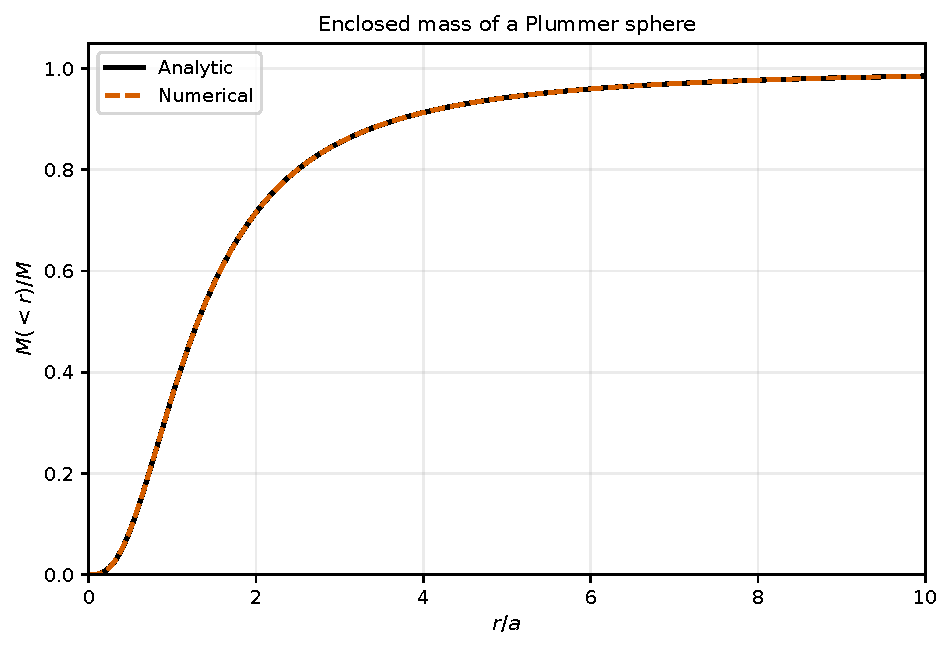
\includegraphics[width=0.68\linewidth]{ch01_enclosed_mass.pdf}
\caption{Plummer 球の内包質量。台形則による累積数値積分と解析解を比較している。計算は $r_{\max}=20a$ まで行い、図は $r\le10a$ の範囲を示す。}
\label{fig:ch1-enclosed-mass}
\end{figure}


\section{内包質量と円運動速度}
\label{sec:ch1-circular-speed}

球対称系では Newton の球殻定理（shell theorem）により、半径 $r$ における重力加速度は、その半径より内側の質量 $M(<r)$ だけで決まる。
ここで $G$ は万有引力定数、$g_r$ は重力加速度の動径成分とし、動径方向は外向きを正に取る。
このとき
\begin{equation}
 g_r(r)=-\frac{GM(<r)}{r^2}
\label{eq:ch1-spherical-gravity}
\end{equation}
である。

半径 $r$ の円軌道を速さ $v_{\rm circ}$ で運動する粒子の半径方向加速度は
\begin{equation}
 a_r=-\frac{v_{\rm circ}^2}{r}
\end{equation}
である。
円運動では、この加速度を重力が与えるので $a_r=g_r$ である。したがって、
\begin{equation}
 -\frac{v_{\rm circ}^2}{r}
 =-\frac{GM(<r)}{r^2}
\end{equation}
となり、
\begin{equation}
 \boxed{
 v_{\rm circ}(r)
 =\sqrt{\frac{GM(<r)}{r}}
 }
\label{eq:ch1-circular-speed}
\end{equation}
を得る\cite{ryden2025}。
式\eqref{eq:ch1-circular-speed}は $r>0$ について書いた式である。
Plummer 球では中心付近で $M(<r)\simeq M(r/a)^3$ なので、$v_{\rm circ}\simeq \sqrt{GM/a^3}\,r$ となり、$r\rightarrow0$ で $v_{\rm circ}\rightarrow0$ である。
Notebook 1 では、この極限に対応して $r=0$ の値を0として扱う。
円運動速度を半径の関数として表したものを\textbf{回転曲線（rotation curve）}と呼ぶ。
したがって、数値積分によって $M(<r)$ が得られれば、式\eqref{eq:ch1-circular-speed}から回転曲線を計算できる。

Plummer 球では内包質量の解析式も分かっているため、回転曲線を解析的に求めることもできる。
式\eqref{eq:ch1-plummer-mass-exact}を式\eqref{eq:ch1-circular-speed}に代入すると、
\begin{equation}
 v_{\rm circ}^2(r)
 =\frac{GMr^2}{(r^2+a^2)^{3/2}}
\label{eq:ch1-plummer-vc}
\end{equation}
となる。
この解析式は、数値積分で得た $M(<r)$ から計算した回転曲線を検証する基準として使える。

ここで、速度の単位を
\begin{equation}
 v_\ast\equiv\sqrt{\frac{GM}{a}}
\label{eq:ch1-velocity-unit}
\end{equation}
とし、無次元半径 $x=r/a$ を導入する。
式\eqref{eq:ch1-plummer-vc}は
\begin{equation}
 \frac{v_{\rm circ}^2}{v_\ast^2}
 =\frac{x^2}{(1+x^2)^{3/2}}
\label{eq:ch1-plummer-vc2}
\end{equation}
となる。
Notebook 1 では $G=M=a=1$ としているため、$v_\ast=1$ である。
物理単位へ戻すには、得られた無次元速度に $v_\ast=\sqrt{GM/a}$ を掛ければよい。

この解析式を使えば、回転曲線が最大となる半径も求められる。
$v_{\rm circ}>0$ なので、$v_{\rm circ}$ を最大にする半径は $v_{\rm circ}^2$ を最大にする半径と同じである。
式\eqref{eq:ch1-plummer-vc2}の右辺を
\begin{equation}
 q(x)=x^2(1+x^2)^{-3/2}
\label{eq:ch1-qx}
\end{equation}
と置く。
微分すると
\begin{equation}
 \frac{dq}{dx}
 =\frac{x(2-x^2)}{(1+x^2)^{5/2}}.
\label{eq:ch1-q-prime}
\end{equation}
$x>0$ で $dq/dx=0$ を満たすのは $x=\sqrt{2}$ である。
導関数はこの点の前後で正から負に変わるため、円運動速度が最大となる半径は
\begin{equation}
 r_{\rm peak}=\sqrt{2}\,a
\label{eq:ch1-vc-peak-radius}
\end{equation}
である。
このとき
\begin{equation}
 \frac{v_{\rm peak}^2}{GM/a}
 =\frac{2}{3\sqrt{3}},
 \qquad
 \frac{v_{\rm peak}}{\sqrt{GM/a}}
 =\sqrt{\frac{2}{3\sqrt{3}}}
 =\choneVcPeakAnalytic.
\label{eq:ch1-vc-peak-value}
\end{equation}

\begin{notebookblock}{1｜円運動速度}
数値積分で得た内包質量 $M(<r)$ から式\eqref{eq:ch1-circular-speed}を用いて回転曲線を計算し、Plummer 球の解析式と比較する。
また、数値的な回転曲線が最大となる格子点を求め、解析値 $r_{\rm peak}=\sqrt{2}\,a$ と比較する。

{\sffamily\small\color{graytext}対応セル（計算部分）}
\begin{Verbatim}[xleftmargin=2mm,fontsize=\small,frame=single,framesep=1.8mm,framerule=0.35pt,rulecolor=\color{listingframe},fillcolor=\color{listingbg}]
# 数値積分で得た M(<r) から円運動速度を求める
vc_num = vcirc_from_mass(r, m_num, G)

# 解析的な M(<r) から求めた円運動速度を比較用に用意する
vc_exact = vcirc_from_mass(r, m_exact, G)

# 数値的な回転曲線が最大となる格子点を探す
i_peak = np.argmax(vc_num)
print(f"数値解の最大位置: r/a = {r[i_peak] / a:.4f}, v_circ = {vc_num[i_peak]:.6f}")

# 解析的な最大位置 r_peak/a = sqrt(2) も表示する
print(f"解析的な最大半径 sqrt(2) = {np.sqrt(2.0):.6f}")
\end{Verbatim}

{\sffamily\small\color{graytext}実行結果}
\begin{Verbatim}[numbers=none,fontsize=\small]
数値解の最大位置: r/a = 1.4035, v_circ = 0.620347
解析的な最大半径 sqrt(2) = 1.414214
\end{Verbatim}
\end{notebookblock}

図\ref{fig:ch1-circular-speed}では、数値積分で得た内包質量から計算した回転曲線と解析式を比較している。
両者はよく一致しているが、400格子点の計算で求めた最大位置は
\begin{equation}
 r_{\rm peak,num}/a=\choneVcPeakRadiusNumerical
\label{eq:ch1-vc-peak-numerical}
\end{equation}
となり、解析値 $\sqrt{2}=\choneVcPeakRadiusAnalytic$ から少しずれる。
これは回転曲線そのものの誤差だけでなく、最大位置を連続的に探索せず、離散的な格子点の中から最大値を選んでいるためである。
より正確な最大位置が必要な場合は、最大付近を補間するか、1変数の最適化を用いる必要がある。

\begin{figure}[!htbp]
\centering
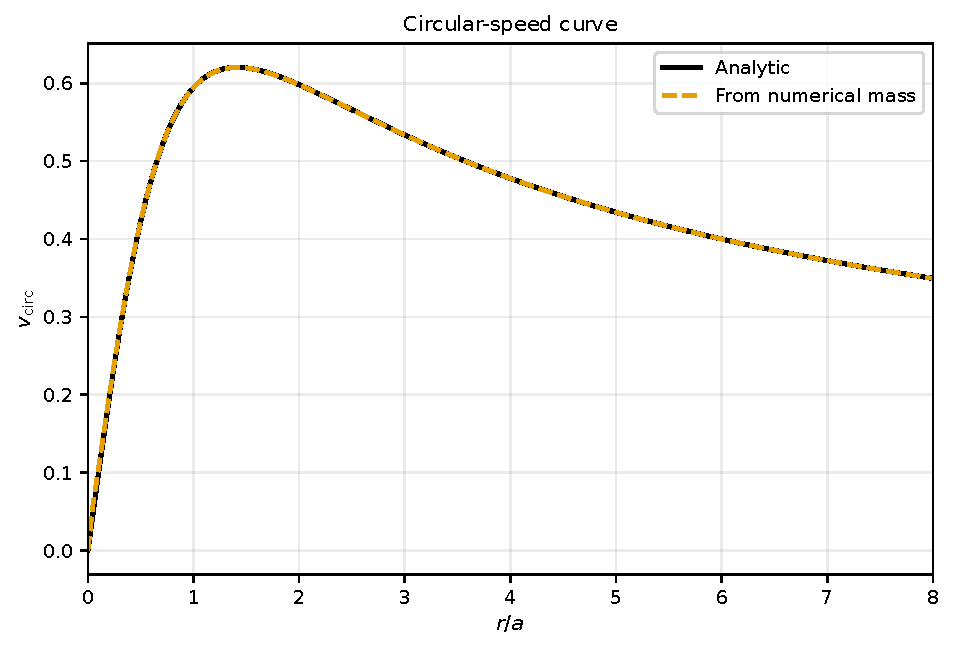
\includegraphics[width=0.68\linewidth]{ch01_circular_speed.pdf}
\caption{Plummer 球の回転曲線。縦軸は $v_\ast=\sqrt{GM/a}$ を単位としている。数値積分で得た内包質量から計算した回転曲線は解析式とよく一致する。解析的な最大位置は $r=\sqrt{2}a$ である。}
\label{fig:ch1-circular-speed}
\end{figure}

\begin{topicblock}{高次元の積分とモンテカルロ積分}
ここまでで、本章で扱う1次元数値積分とその物理的応用は完結した。
最後に、積分の次元が高くなると計算量と誤差の関係がどのように変わるかを簡単に見ておく。

本章では、積分区間を格子に分け、台形則や Simpson 則で1次元の定積分を求めた。
1次元で誤差が $h^p$ で減る積分公式では、滑らかな関数に対して格子を細かくするほど急速に精度が上がる。

一方、$d$ 次元の積分で各方向を $n$ 分割すると、総評価点数はおよそ $N_{\rm eval}=n^d$ になる。
1次元の積分公式を各方向に同じように適用すると、$h\sim N_{\rm eval}^{-1/d}$ なので、誤差はおおよそ
\[
 \epsilon\sim N_{\rm eval}^{-p/d}
\]
で減る。したがって、次元が高くなるほど、同じ評価点数で得られる精度は低下する。

これに対して、積分領域から無作為に点を選び、被積分関数の平均値から積分値を推定する方法を
\textbf{モンテカルロ積分（Monte Carlo integration）}という。区間 $[x_{\min},x_{\max}]$ では
\[
 I=\int_{x_{\min}}^{x_{\max}} f(x)\,dx
 \simeq
 \frac{x_{\max}-x_{\min}}{N_{\rm samp}}\sum_{k=1}^{N_{\rm samp}}f(x_k)
\]
と見積もる。ここで $x_k$ は区間内から独立に、一様に選んだ点であり、$N_{\rm samp}$ はサンプル数である。
被積分関数の分散が有限なら、この推定値の標準誤差は $N_{\rm samp}^{-1/2}$ に比例して減り、その指数は積分の次元に直接依存しない。
したがって、1次元の滑らかな積分では本章の方法のほうがはるかに効率的である。
一方、次元が高い場合や積分領域の形が複雑な場合には、モンテカルロ積分が有力な選択肢になる。
天文学では、輻射輸送でも乱数によるサンプリングが利用されている\cite{matsumoto}。

重力多体系シミュレーションで、等質量粒子の初期位置を作るときにも、乱数と内包質量を使う。
球対称分布の全質量を $M$ とし、$0<X<1$ の一様乱数を生成して $M(<r)/M=X$ を満たす半径 $r$ を求める。
この操作を\textbf{逆関数法（inverse transform sampling）}という。
半径の確率密度は $\rho(r)$ そのものではなく $4\pi r^2\rho(r)/M$ であり、方向も等方的に選ぶことで、密度分布 $\rho(r)$ に対応する粒子配置を作れる。
Plummer 球では式\eqref{eq:ch1-plummer-mass-exact}を逆に解き、
\[
 r=a\left(X^{-2/3}-1\right)^{-1/2}
\]
と求められる。
一般の密度分布では、累積積分で得た内包質量の表を逆にたどり、必要に応じて補間して半径を決める。
有限半径 $r_{\max}$ までの表を使う場合は、その半径までの質量で規格化し、$M(<r)=X M(<r_{\max})$ を満たす半径を求める。
これは位置分布の作成であり、平衡な初期条件を作るには、質量分布と整合する速度分布も別途与える必要がある。
粒子を独立に抽出すると、一定の半径内に入る粒子数の割合には統計的なゆらぎが残る。
その標準偏差は粒子数 $N_{\rm p}$ に対して $N_{\rm p}^{-1/2}$ に比例する。
これは乱数サンプリングのゆらぎであり、累積積分の離散化誤差や、その後の時間積分の誤差とは区別する。

詳しくは、乱数とモンテカルロ法は三井田・須田\cite{miida2023}第9章、
重力多体系の計算は富阪ほか編\cite{tomisaka2007}第6章を参照すること。
\end{topicblock}

